\subsection{Geometry}

\paragraph{}
Arguably the most important parts of the input file are the cards defining the configuration space— namely the detector and media with respect to the cartesian coordinate system. In FLUKA this is known as the \textit{geometry}. The geometry section of the input card is demarcated by \textbf{GEOBEGIN} and \textbf{GEOEND} cards. Between these two cards are first cards for various \textit{bodies} which are basic 2D and 3D geometric surfaces, and second, cards for \textit{regions} whose bounds are defined by combinations of geometric \textit{bodies}. For instance, a triad of bodies could be a cylinder whose axis lies on the $z$-axis, and two planes lying parallel the $x-y$ plane at different $z$s. A region defined by these bodies could be the 3D cylindrical volume made by the cylinder body capped off on either end by the two planes. This is exactly the type of region representing the nEXO OD and the nEXO TPC. 

\begin{figure}[h]
    \begin{center}
    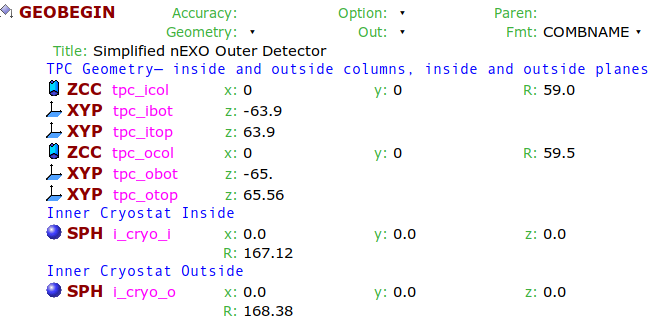
\includegraphics[scale=0.5]{figures/geometry_1.png}
    \caption{An example of the geometry body declarations in the input file}
    \label{fig:geometry1}
    \end{center}
\end{figure}

\paragraph{}
Figure \ref{fig:geometry1} shows the first part of the geometry declarations in the nEXO input file. We see the first card is the \textbf{GEOBEGIN} with the argument \textit{fmt} set to COMBNAME. This tells the FLUKA binaries how to read in the following geometry cards. This is not particularly important. This seems to be the default mode. Text in \textcolor{blue}{blue} indicates a comment (equivalent to a FORTRAN77 comment in the input file) and body variable names are in \textcolor{magenta}{pink} and are limited to lengths of 8 characters. The names or types of cards are fully capitalized and in \textcolor{Maroon}{maroon}. The argument names for each card are written in \textcolor{ForestGreen}{green} and the arguments follow with an 8 character length limit. These colour conventions hold for every other type of input card. Each card can have many arguments, but generally, not all are necessary. In the geometry body cards however, each argument is provided as these arguments are all necessary to uniquely define their respective geometric body. For instance, there is a body called \textcolor{magenta}{i\_cryo\_i} defined with a \textcolor{Maroon}{SPH} card. The name is intented to be shorthand for ``inner cryostat inside'' and, being a sphere, requires a radius and three coordinates for its location in space. There are many choices for bodies in FLUKA, each of which fairly simple to define.

\paragraph{}
Regions, as previously discussed, are created with logical combinations of bodies. Imagine the bodies defining surfaces in 3D, and the regions being the volumes they surround. Following the set of cards defining the bodies, there is an \textbf{END} card, then the region cards as shown in figure \ref{fig:geometry2}, finally there is the \textbf{GEOEND} card. Each region must be assigned \textbf{one} material— we'll get to material assignments later. For example, the region inside the nEXO OD that is full of water would be defined by the OD inside body minus the outer cryostat outside body leaving the configuration of a cylinder with a spherical hole in its volume— the entirety of this region is to be water. 

\begin{figure}[h]
    \begin{center}
    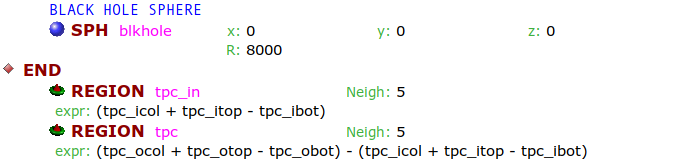
\includegraphics[scale=0.5]{figures/geometry_2.png}
    \caption{An example of the geometry region declarations in the input file}
    \label{fig:geometry2}
    \end{center}
\end{figure}

\paragraph{}
Looking at figure \ref{fig:geometry2}, we see the final body declaration followed by the first few region declarations in the nEXO input file. The final body here is important— each FLUKA configuration defines its physical boundaries by assigning material \textit{blackhole} to its outermost surface- hence the name of the sphere. The first region we have defined is \textcolor{magenta}{tpc\_in} will be the inside of the TPC cylinder— the part filled with liquid xenon. While no number is assigned by the user to the region, FLUKA assigns it number 1 as it is the first defined- this will be important later. The construction of the region is in the \textcolor{ForestGreen}{expr} argument given by ``(tpc\_icol $+$ tpc\_itop $-$ tpc\_ibot)''. We first have \textit{tpc\_icol} which is the inside cylinder (along $z$) of the TPC which alone is unbound and spans the entire $z$-axis. To the cylinder we add \textit{tpc\_itop} (xy-plane) which sets the upper bound, and subtract \textit{tpc\_ibot} (xy-plane) which sets the lower bound. This process is similar for all other region declarations. Unfortunately, one may not reference regions by name in region expressions, only bodies; hence the following region declaration of the \textcolor{magenta}{tpc} which is intended to be the material composing the TPC. The \textcolor{ForestGreen}{Neigh} argument is an integer which defines ``neighbourhoods'' relating regions to each other. This can perhaps be deployed for larger, more complex geometries but given the simplicity of the nEXO OD geometry and the lack of thorough documentation of this feature, it has been set to the default value of 5 for each region. Once more, the \textbf{GEOEND} card (not shown) brings us to the end of the geometry card section.

\subsubsection{The Chosen Configuration}
\paragraph{}
The simulations performed here deployed a simplified geometry of nEXO. There were no PMTs included, no complicated internal structure and no contoured cavernous room around the detector. It is simply a large stainless steel cylinder surrounded by norite rock \cite{olivia_scallon} and full of water containing the inner and outer cryostats and the copper TPC filled with liquid Xenon-136. That's it. The masses for the TPC and the cupric TPC shell were chosen to correspond with parallel GEANT4 simulations. This is an important consideration for scoring activation of particular isotopes. The muons are propagated through at least 15m of rock before reaching the detector, and the rock surrounding the OD laterally is 20m, and below it, 5m. Where possible, the measurements for the configuration were taken from the ``nEXO Preliminary Design Report'' except for the size of the OD which has been adjusted to meet the more recent specification.

\begin{figure}[h]
    \begin{center}
    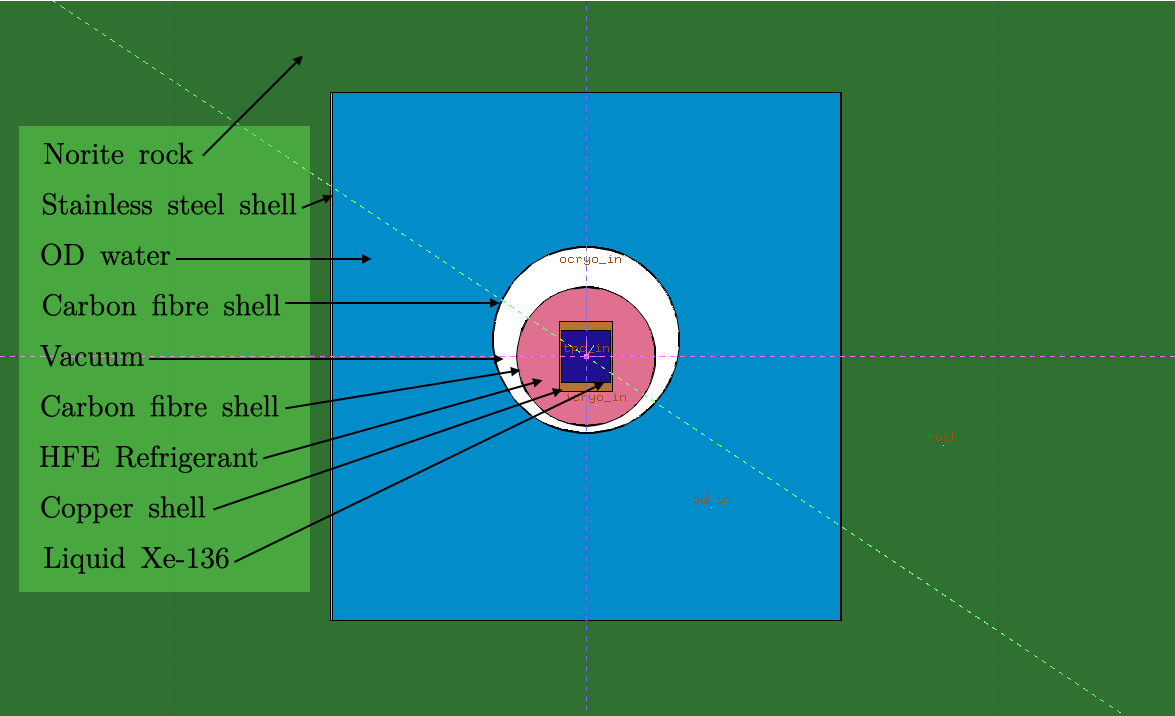
\includegraphics[scale=0.3]{figures/geometry_3.png}
    \caption{A 2D projection of the nEXO geometry used in the FLUKA simulations}
    \label{fig:geometry3}
    \end{center}
\end{figure}